\section{Ristoratore}
Oltre alle funzionalità presenti come ospite, un ristoratore può effettuare 
le seguenti azioni:
\begin{itemize}
    \item Accedere alla propria area personale (My Area)
    \item Scrivere recensioni sui ristoranti
    \item Creare nuovi ristoranti
    \item Gestire i ristoranti creati
    \item Rispondere alle recensioni dei propri ristoranti
\end{itemize}

\subsection{Area Privata Ristoratore}
Premendo sul pulsante \emph{My Area} in alto a destra nella schermata 
di ricerca (Figura~\ref{fig:search}), l'utente accede alla propria area personale.\\
In questa schermata l'utente può visualizzare:
\begin{itemize}
    \item Numero di ristoranti di cui è proprietario in alto a sinistra
    \item Qual è il punteggio medio delle recensioni dei propri ristoranti
    \item Il numero di ristoranti recensiti
    \item Elenco dei ristoranti gestiti a sinistra
    \item Elenco delle recensioni scritte a destra
    \item In alto a destra un pulsante \emph{Logout} per tornare alla schermata di login (Figura~\ref{fig:login})
    \item In alto a destra, a fianco del pulsante di Logout, 
    un pulsante \emph{Back to Search} per tornare alla 
    schermata di ricerca (Figura~\ref{fig:search})
\end{itemize}
\begin{figure}[H]
    \centering
    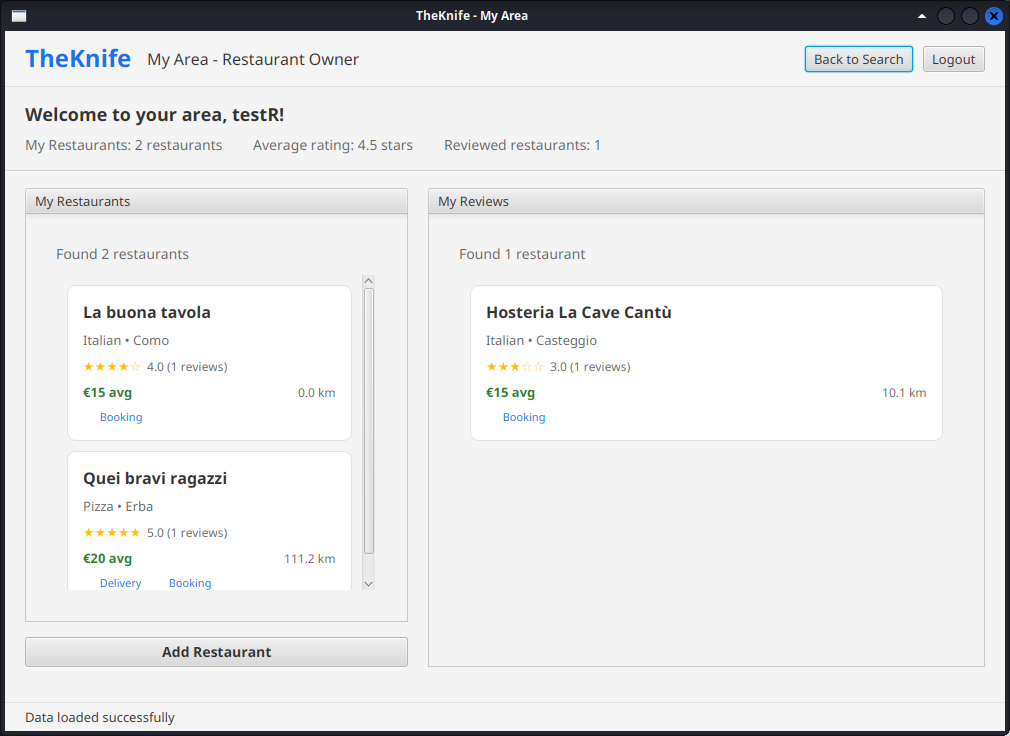
\includegraphics[width=0.8\textwidth]{images/myarea-owner.png}
    \caption{Schermata Area Privata Ristoratore}
    \label{fig:myarea-owner}
\end{figure}
Da questa schermata l'utente può agevolmente gestire i suoi ristoranti.
\paragraph{Nota}
Le modifiche effettuate nella propria area 
personale non sono immediatamente visibili. Occorre uscire 
dalla propria area personale e rientrare per visualizzare 
le modifiche apportate.
\subsection{Creazione ristorante}
Per aggiungere un nuovo ristorante, premere il pulsante \emph{Add Restaurant} (Figura~\ref{fig:myarea-owner}).
Verrà mostrata una schermata apposita per la creazione del ristorante (Figura~\ref{fig:add-restaurant}).
Il ristoratore è tenuto a compilare tutti i campi.
\begin{figure}[H]
    \centering
    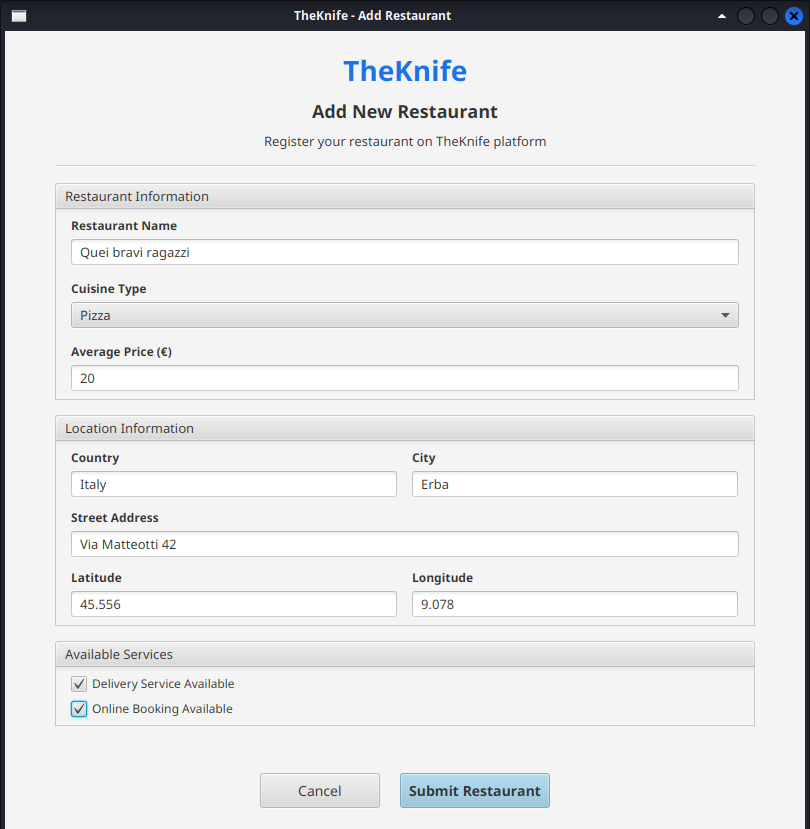
\includegraphics[width=0.8\textwidth]{images/add-restaurant.png}
    \caption{Interfaccia per la creazione di un ristorante}
    \label{fig:add-restaurant}
\end{figure}
Una volta compilato il form, premere il pulsante \emph{Submit Restaurant} per creare il ristorante.

\subsection{Recensioni}
Dalla vista del dettaglio del ristorante (Figura~\ref{fig:restaurant})
l'utente può scrivere una recensione premendo il pulsante 
\emph{Write a Review}. 
Una volta premuto il pulsante comparirà una schermata per scrivere 
la propria recensione.\\
Selezionare un punteggio da 1 a 5 premendo sulla stella corrispondente
il punteggio che si desidera assegnare.
Se lo si desidera, scrivere un commento nella casella di testo.
Il commento è facoltativo, ma è consigliato per rendere la recensione
più utile agli altri utenti.\\
Le recensioni possono essere modificate o cancellate in qualsiasi 
momento dalla propria area personale (Figura~\ref{fig:myarea-client}).
\begin{figure}[H]
    \centering
    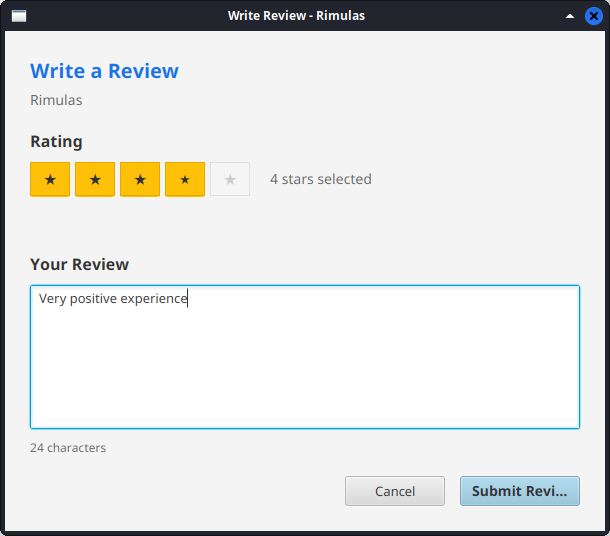
\includegraphics[width=0.8\textwidth]{images/review.png}
    \caption{Schermata di scrittura recensione}
    \label{fig:review}
\end{figure}
\paragraph{Note}
\begin{itemize}
    \item Il ristoratore non può scrivere recensioni a ristoranti di cui è 
    proprietario.
    \item Il commendo non può eccederei i 255 caratteri.
\end{itemize}

\subsection{Risposte alle recensioni}
Premendo su un ristorante di cui si è proprietari, l'utente può 
visualizzare le recensioni ricevute (Figura~\ref{fig:restaurant}).\\
I ristoratori possono rispondere alle recensioni dei propri locali premendo 
sulla recensione a cui si desidera rispondere nell'elenco delle recensioni ricevute.
Verrà mostrata una schermata apposita per la gestione della risposta (Figura~\ref{fig:reply}).
Una volta scritta la risposta, premere il pulsante \emph{Submit Reply} o 
\emph{Update Reply} per inviare o modificare la risposta.
\begin{figure}[H]
    \centering
    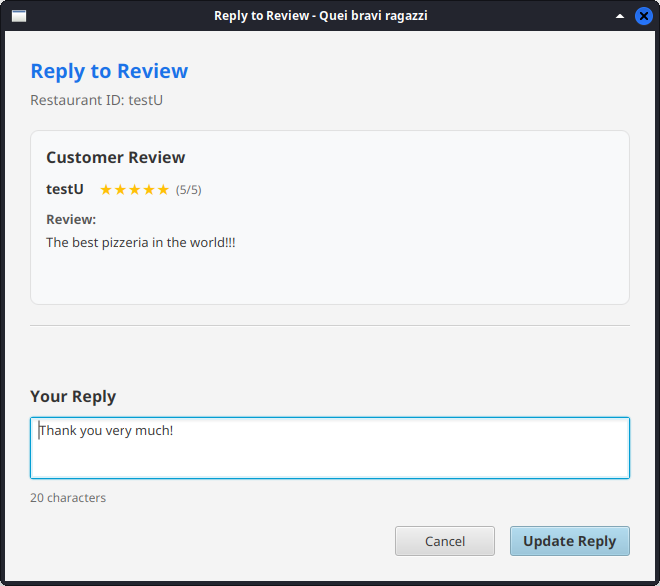
\includegraphics[width=0.8\textwidth]{images/reply.png}
    \caption{Interfaccia per la gestione delle risposte}
    \label{fig:reply}
\end{figure}
\paragraph{Note}
\begin{itemize}
    \item La risposta non può eccedere i 255 caratteri.
    \item Se la recensione viene cancellata o modificata dal cliente,
    la risposta verrà automaticamente cancellata.
\end{itemize}
